%% LyX 2.1.1 created this file.  For more info, see http://www.lyx.org/.
%% Do not edit unless you really know what you are doing.
\documentclass[english]{article}
\usepackage[T1]{fontenc}
\usepackage[latin9]{inputenc}
\usepackage{geometry}
\geometry{verbose,tmargin=1in,bmargin=1in,lmargin=1in,rmargin=1in}
\usepackage{float}
\usepackage{amsmath}
\usepackage{graphicx}

\makeatletter

%%%%%%%%%%%%%%%%%%%%%%%%%%%%%% LyX specific LaTeX commands.
%% Because html converters don't know tabularnewline
\providecommand{\tabularnewline}{\\}

\makeatother

\usepackage{babel}
\begin{document}

\title{Lab 4: Cloud Data\\
Stat 215A, Fall 2014}


\author{Russell Chen, Sreeta Gorripaty, Mo Zhou}

\maketitle

\section{Introduction}

In this report, we explore  cloud detection in the polar regions based on radiances of three images recorded automatically by the MISR sensor aboard the NASA satellite Terra. The classification of cloud and non-cloud is a difficult problem to solve in snow covered regions, due to similarity of cloud and snow cover. In this report, we explore the data using exploration techniques such as k-means, random forests and density plots of the variables. After getting a good idea of the behavior of the image data, we select the important features to create a classification model to identify clouds from non-clouds. For the purpose of classification, we only consider the cloud and non-clouds and discard the not-sure data points. We test out our models against the ?expert labels? for cloud classification to assess the prediction. \\
\\
The data we have consists of three images from the MISR sensor. For each image, we have the x,y coordinates of pixels, the expert label of the pixels, the radiances from five different angles and three features associated with the pixels, namely NDAI, SD and CORR. The CORR feature is developed by measuring the correlation across the pixels from different angles of image over a patch of the image. The SD feature measures the standard deviation of the radiation from the five angles over a patch of image. NDAI measures the gradient across different patches of the image. The main point that we exploit here is that for non-clouds the same point is captured form different angles and thus the radiation from different angles is similar. We aim to use these information to develop a classification model that can predict for cloud.


\section{Exploratory Data Analysis}


\subsection{Plots of expert labels for the presence or absence of clouds}

\begin{figure}[H]
\begin{centering}
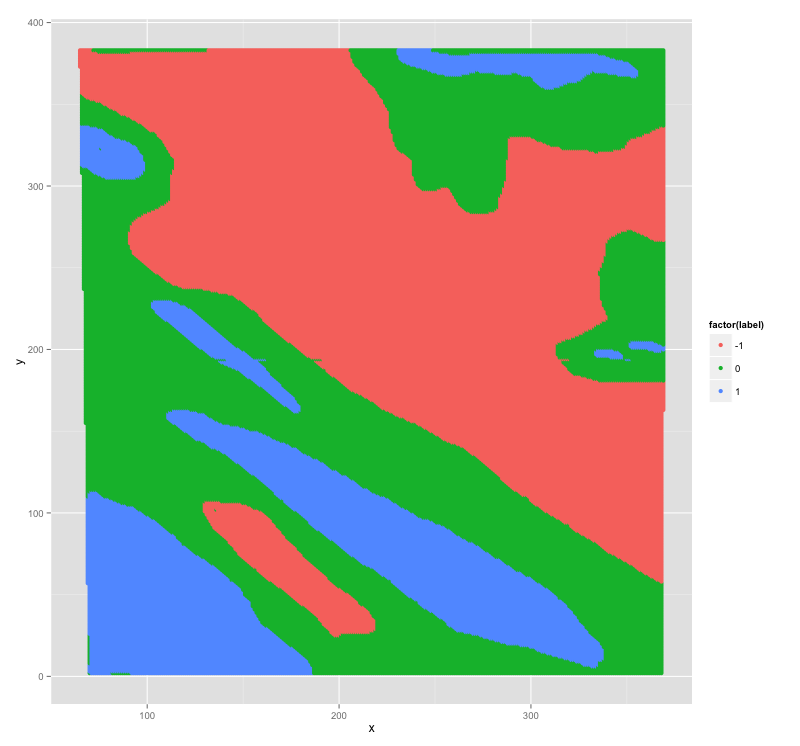
\includegraphics[scale=0.2]{plot/image1}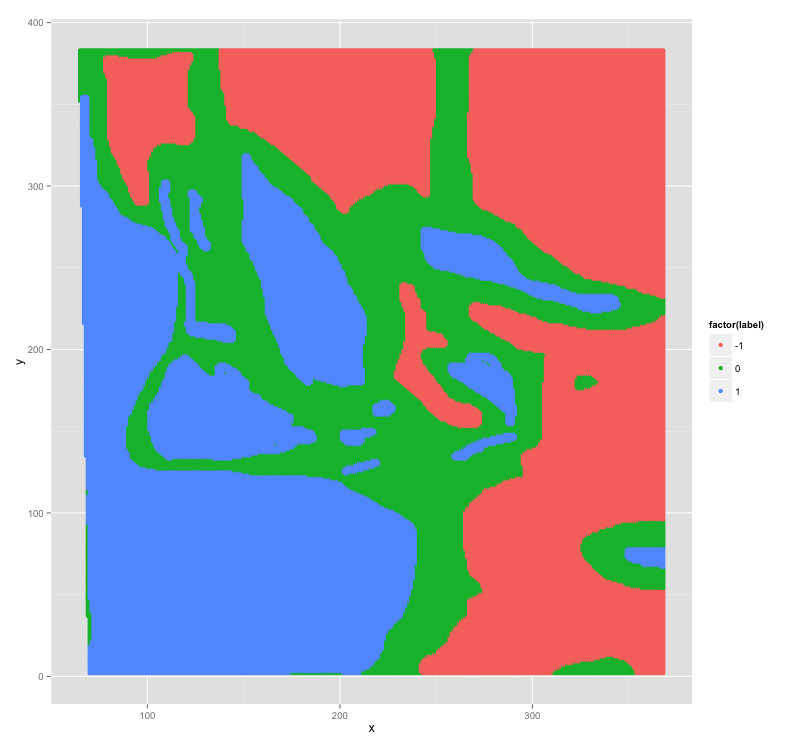
\includegraphics[scale=0.2]{plot/image2}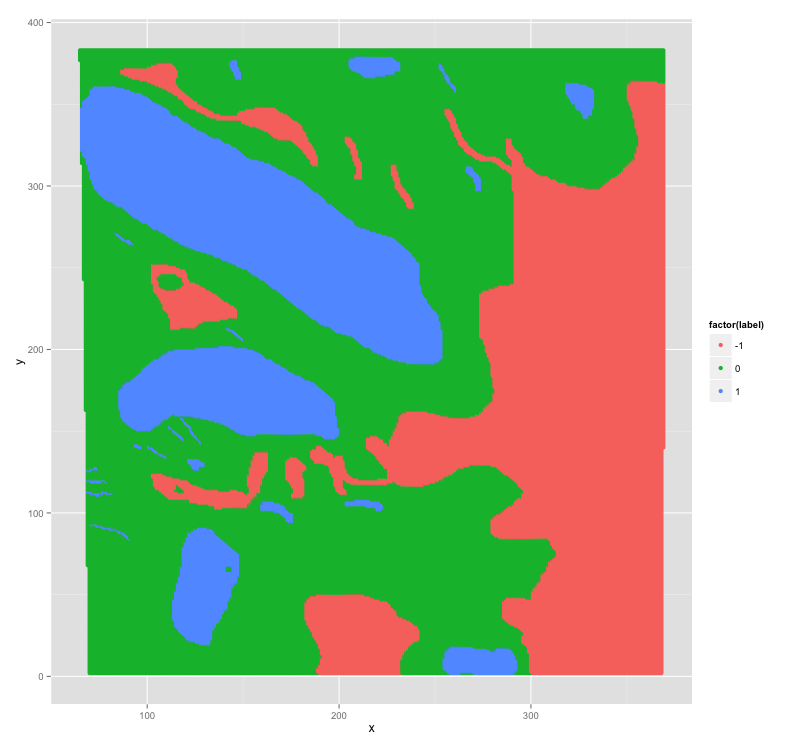
\includegraphics[scale=0.2]{plot/image3}
\par\end{centering}

\protect\caption{The expert labels of the three images. 1 indicates cloud, -1 indicates
no cloud, 0 indicates not sure.}


\end{figure}
There are clustering of cloud and non-cloud for the three images,
i.e. the pixels next to some cloud pixel tend to be cloud as well.
We also observe that image3 looks different from the other images
because it has several small regions of cloud/ non-cloud.


\subsection{Radiances of Different Angles}

The radiances of different angles are similar among the three images.
Here we use image1 as an example. The plots below show that the radiances
of different angles do not indicate significant differences. The general
shapes of the plots are alike and there is no clear difference visually.
Density plots of radiances of different angles colored by labels are
shown on the next page.\\


\begin{figure}[H]
\noindent \begin{centering}
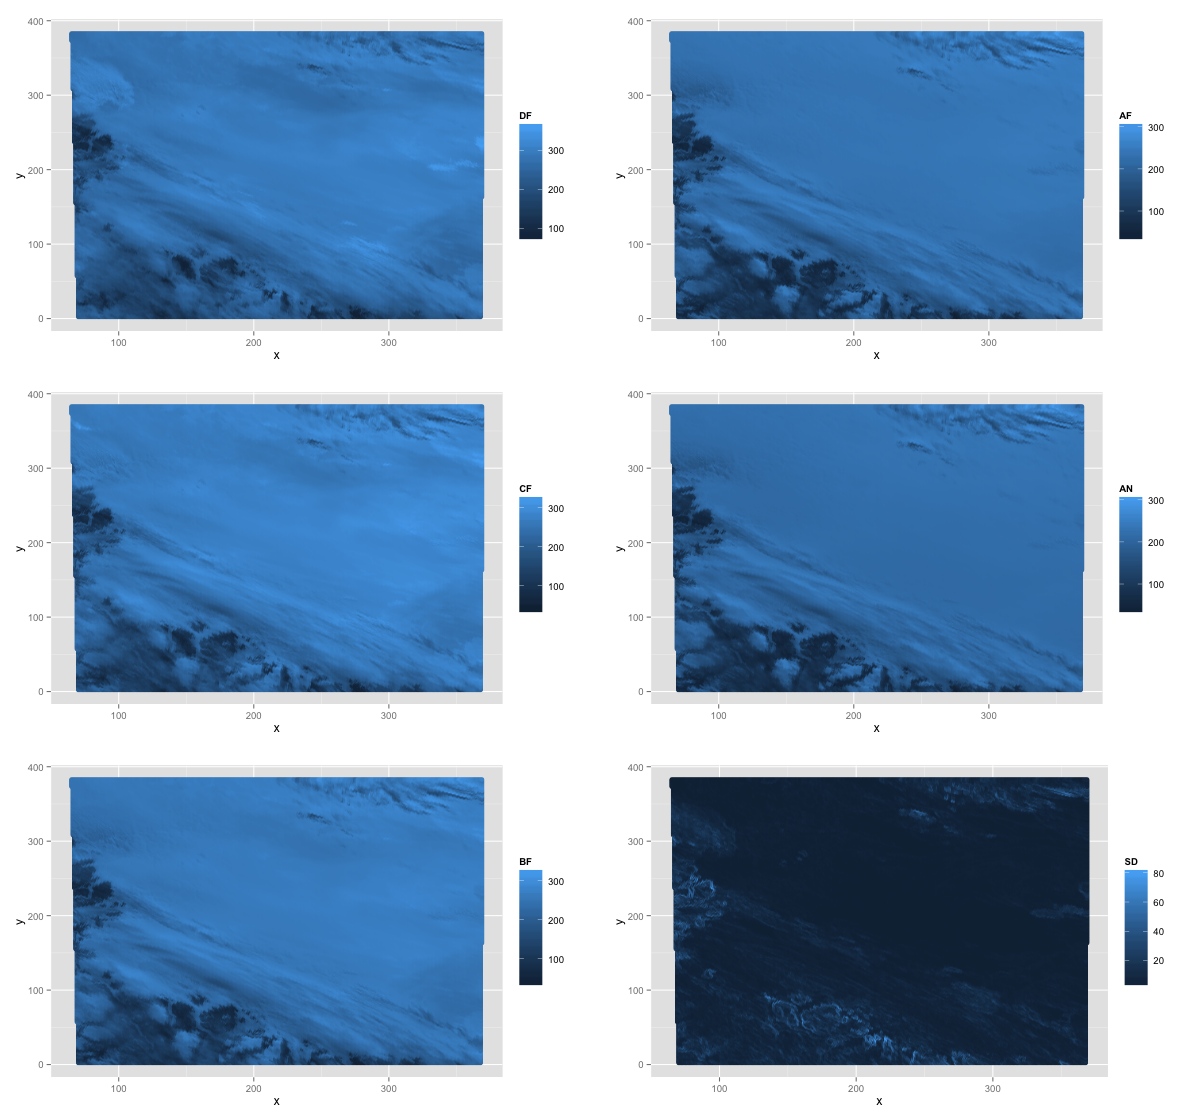
\includegraphics[scale=0.4]{plot/multiangleimage1}\protect\caption{Radiances of different angles of image1}

\par\end{centering}

\end{figure}


\newpage{}
\begin{figure}[H]
\centering{}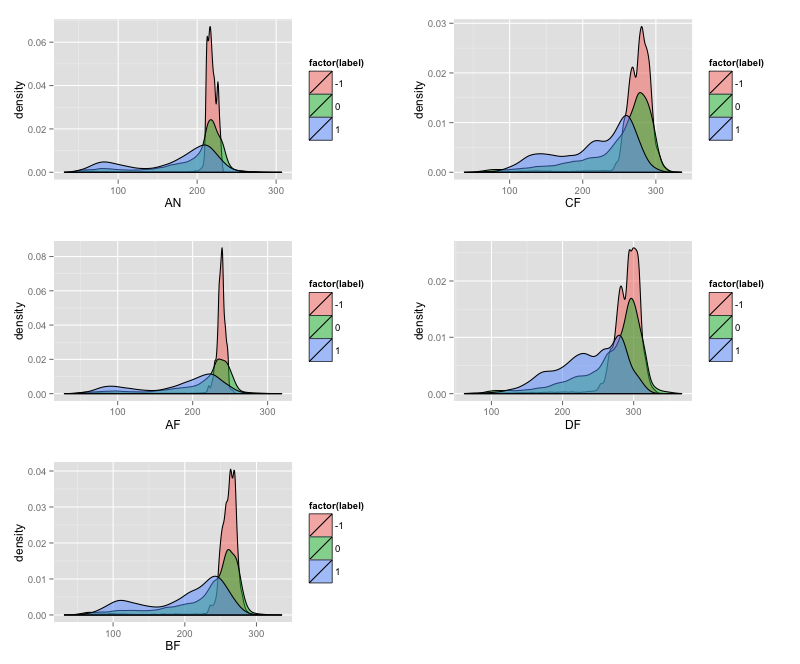
\includegraphics[scale=0.55]{plot/multidensity}\protect\caption{Densities plot of labels with radiances of different angles.}
\end{figure}

\noindent
There are no clear intervals that split the labels based on the radiance
variables. Thus it is hard to determine if some pixel is cloud just
based on the radiance information from different angles. However,
we see that the three features provides us better information in classifiying
the cloud information from non-cloud. The density plots are shown
below:\\
\\
\begin{figure}[H]


\begin{centering}
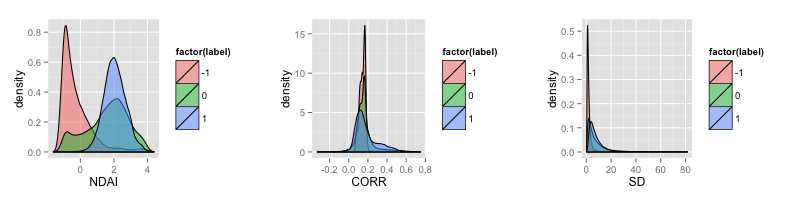
\includegraphics[scale=0.5]{plot/densityfeature}\protect\caption{Densities plot of labels with features NDAI, CORR, SD respectively}

\par\end{centering}

\end{figure}

\noindent
The density plot of NDAI shows a clear difference in values associated
with different labels, which indicates a big difference based on NDAI
and suggests that NDAI would be a useful feature to include when deciding
the classification of cloud. The differences based on CORR and SD
are not as evident as NDAI, but are still more informative than the
radiances, so we might want to consider these two features as well
in the classification models.\\



\subsection{Unsure labeling treatment}

In the images, all pixels are classified by the expert into three
groups: cloud, non-cloud and unsure. The pixels with not sure labels
are not informative in our classification of cloud, nor is it valuable
for us to predict for them. Thus in our analysis and models below,
we disregard all the pixels with unsure labeling and are only concerned
with the pixels with clear cloud/non-cloud labeling. 


\section{Feature selection}


\subsection{Three best features by density plot}

As shown in our exploratory data analysis, the density plot provides
us valuable information about the different feature values corresponding
to the labels. It shows that NDAI demonstrates the most clear split
of the two classes and would be the best feature to consider in the
classification models. CORR and SD are important features because
some interval of these observations belongs to some particular class.
Thus we propose that NDAI, CORR and SD are the best features we wish
to include in our classification models.


\subsection{K-Means clustering based on the three features}

To confirm how well the features could predict the classes of our
data, we carry out K-Means clustering method on the three images and
the three features respectively to obtain the following True Positive
Rate (TPR) and False Positive Rate (FPR) results:\\


\begin{center}
\begin{tabular}{|c|c|c|c|}
\hline 
 &  & TPR & FPR\tabularnewline
\hline 
\hline 
 & NDAI & 0.9775292 & 0.1112675\tabularnewline
\cline{2-4} 
Image 1 & CORR & 0.2122026 & 0.01879237\tabularnewline
\cline{2-4} 
 & SD & 0.2648136 & 0.03475003\tabularnewline
\hline 
 & NDAI & 0.9943717 & 0.1236416\tabularnewline
\cline{2-4} 
Image 2 & CORR & 0.4620028 & 0.009304603\tabularnewline
\cline{2-4} 
 & SD & 0.1918963 & 0.02663122\tabularnewline
\hline 
 & NDAI & 0.9416306 & 0.2492889\tabularnewline
\cline{2-4} 
Image 3 & CORR & 0.5050838 & 0.05211543\tabularnewline
\cline{2-4} 
 & SD & 0.2305592 & 0.05288575\tabularnewline
\hline 
\end{tabular}
\par\end{center}


\subsection{Random forest for feature selection}

After discarding all the 'unsure' labels, we combined the 3 images
and fit a random forest to the data. This allowed us to rank the variables
in order of importance for prediction. The \texttt{randomForest} package
in R calculates variable importance in 2 ways and plots the results,
as shown. \\
\\
\begin{figure}[H]
\begin{centering}
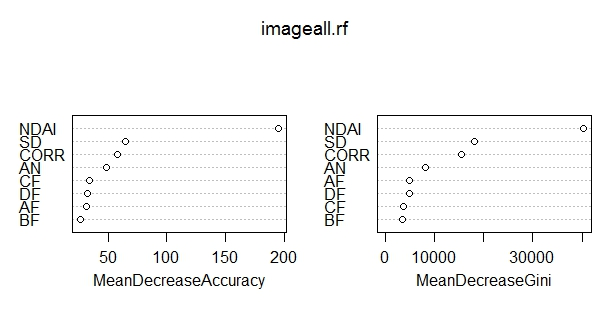
\includegraphics[scale=0.5]{plot/varImp.jpeg}
\par\end{centering}

\protect\caption{Variable Importance plots generated by Random Forest}


\end{figure}
\noindent
On the left, the variables are ranked according to a permutation importance
measure. To compute this importance measure for a variable $p$, for
each tree grown in the random forest, the classification error rate
is computed for out-of-bag (OOB) data points in two cases. The first
case is where all the variables in the OOB data points are left untouched.
The other case is where the values of variable $p$ are randomly permuted.
The classification error rate on the OOB data points for these two
cases is compared and the difference between them averaged across
all trees to compute a permutation importance measure. A larger difference
in the respective classification error rates indicates a variable
that has larger predictive power and is therefore more important.\\
\\
On the right, the variables are ranked according to Gini importance.
The Gini index is a measure of dispersion for a list of numbers. Smaller
values of the Gini index indicate greater equality and vice versa.
In a decision tree, for each split on variable $p$, the Gini index
for each descendent node is lower than that of the parent node. The
larger the Gini index decreases for each split, the better variable
$p$ is at separating the classes and therefore more important for
classification.\\
\\
The two plots shown consistently rank NDAI, SD and CORR as the 3 most
important variables for the purposes of prediction. This is also consistent
with our earlier reasoning about the importance of NDAI, SD and CORR.


\section{Classification}


\subsection{Linear Discriminant Analysis (LDA)}

LDA models each class (cloud or non-cloud) as a multivariate Normal
distribution of the predictor variables and assumes that both classes
have the same covariance matrix $\varSigma$. These are the class-conditional
densities. 
\[
f_{k}(x)=\frac{1}{(2\pi)^{p/2}\mid\Sigma\mid^{1/2}}e^{-\frac{1}{2}\left(x-\mu_{k}\right)^{\mathrm{T}}\varSigma^{-1}\left(x-\mu_{k}\right)}
\]
Establishing prior probabilities on the classes then allows us to
model the posterior probabilities of the classes given the predictor
variables in the data by applying Bayes rule. The parameters $\mu_{k}$
and $\varSigma$ of both Gaussian distributions are estimated from
training data. In this case, the discriminant functions - and therefore
the decision boundaries - are linear in the predictors: 
\[
\delta_{k}(x)=x^{\mathrm{T}}\Sigma^{-1}\mu_{k}-\frac{1}{2}\mu_{k}^{\mathrm{T}}\Sigma^{-1}\mu_{k}+log\pi_{k}
\]
For the LDA models we fitted, the default class priors $\pi_{k}$
were used: empirical proportion of each class in the training set.


\subsection{Quadratic Discriminant Analysis (QDA)}

QDA works in the same fashion as LDA. The class-conditional densities
are multivariate Normal distributions of the predictor variables.
However, unlike LDA, it does not assume that both classes have the
same covariance matrix. The discriminant functions do not simplify;
they are quadratic in the predictors:
\[
\delta_{k}(x)=-\frac{1}{2}log\mid\varSigma_{k}\mid-\frac{1}{2}\left(x-\mu_{k}\right)^{\mathrm{T}}\varSigma_{k}^{-1}\left(x-\mu_{k}\right)+log\pi_{k}
\]
 Parameters $\mu_{k}$ and $\varSigma_{k}$ of both Gaussians are
also estimated from training data. Again, we used the default class
priors due to not having any expert knowledge of cloud cover in the
Arctic.\\
\\
For both LDA and QDA, we did not check the assumptions that the data
is Gaussian because we are interested in prediction instead of inference.
LDA and QDA models may still do reasonably well at prediction despite
the data not being strictly Gaussian. In any case, we will assess
all the classification models with the Area under the ROC curve (AUC),
as discussed later. 


\subsection{Logistic regression}

Since we only have two classes, the logistic regression model consists
of only a single linear function: 
\[
log\frac{P(label=\text{no cloud}|X=x)}{1-P(label=\text{no cloud}|X=x)}=\beta_{0}+\beta_{1}^{\mathrm{T}}x
\]
It is fitted by maximum likelihood in R and the probabilities of each
class given the data can be calculated.


\subsection{Semi-supervised Expectation-Maximization (EM)}

An expectation-maximization (EM) algorithm is an iterative method
for finding maximum likelihood or maximum a posteriori (MAP) estimates
of parameters in statistical models, where the model depends on unobserved
latent variables. Semi-supervised EM has proportion of the latent
variables known to us, but the other proportion unknown to predict.
In our problem, we use the labels of the training set as known latent
variables to predict the labels of the testing set. The predictors
that are concerned in the Semi-supervised EM model are NDAI, CORR
and SD. Other combinations of the variables are also tested, but the
performance is not as good.


\subsection{Support Vector Machine (SVM)}

SVMs are supervised learning models in which a hyper-plane is constructed
to divide the data into its classes. The training dataset is used
to tune its hyper-parameters (gamma and cost) using cross-validation.
From experimentation with the sample sizes of the training dataset,
we observed that SVM is a very computationally expensive classification
method. For our given dataset of 3 images, training on two or one
image did not converge even after running for 2 days.\\
\\
To overcome this problem, we constructed our training dataset by sampling
points in the images meant for training. It is interesting to note
that the very reason why it is not a good practice to choose points
randomly from the images for cross-validation, validates our sampling
approach for SVM. In the cloud identification problem, since neighboring
pixels are correlated, we gain sufficient information about the training
images, by sampling a smaller number of pixels for hyper-parameter
tuning.\\
\\
The hyper-parameters and kernel for the SVM models are chosen from
grid-search and tuning on the training set. The SVM model is trained
on varying sizes of training data, ranging from 5000 pixels to 15000
pixels.


\section{Model Assessment}


\subsection{Cross-validation}

The images we are dealing with are examples of spatially dependent
data. The features of pixels very close to each other are likely to
be very similar. The usual method of doing $k$-fold cross validation
by partitioning the data into $k$ folds uniformly at random is not
ideal since it operates on the assumption that the data points are
independent and data points are exchangeable. Thus, when we randomly
sample points from all our images in cross-validation, we essentially
capture the behavior of larger chunks of data from all the images
due to the correlation of pixels. Essentially, this translates to
our model 'seeing' all the images and our prediction error is underestimated
when we use our classification model on the remaining points of the
three images. However, when we apply our prediction on a new image
that our training model has not seen before, we will end up getting
large prediction errors and poor future prediction.\\
\\
To overcome this problem, we would like to cross validate in a way
that ensures that no data points in folds used for training are close
to data points in the folds used for testing. We briefly considered
dividing each image into 4 patches by cutting at the midpoint of each
of the two coordinate axes and making each patch a single fold in
our $k$-fold cross validation procedure. However, we observed that
training on 11 patches and testing on 1 patch gave extremely unstable
AUCs, with AUCs being very low for 2-3 folds and very high for majority
of the folds. This might be accounted for the fact that the 12th patch
is an 'unseen' image and in some cases, our classification model was
not good for the 12th patch. We experimented with the number of patches
in the testing set to overcome this problem, but this resulted in
an extremely large number of folds leading to expensive computation
and the resulting AUC values are not as good as putting 2 images in
the training set and the other image in the testing set.\\
\\
After comparing the model performance for different number of patches,
we decided to train on 2 images and then test on the other one. We
believe that this is the best simulation of what happens when the
classifier is used to predict on a completely new image, since the
entire third image is 'unseen' by our classification model.


\subsection{Akaike Information Criterion (AIC)}

The value of the AIC is calculated as:
\[
\text{AIC}=2k-2log(L)
\]
 where $k$ is the number of parameters of the model and $L$ is the
maximized value of the likelihood function for the model. AIC deals
with the trade-off between the goodness of fit of the model and the
complexity of the model. It is founded on information theory: it offers
a relative estimate of the information lost when a given model is
used to represent the process that generates the data. We use AIC
to assess the logistic regression models with varied number of variables,
i.e. with only one variable, three variables, or with four variables.
AIC cannot be applied to LDA, QDA because there is no likelihood associated
with those methods. By applying AIC to each fold in CV, we summarized
results in the following table:

\begin{center}
\begin{tabular}{|c|c|c|}
\hline 
Predictors & Fold & AIC\tabularnewline
\hline 
 & 1 & 72739.29\tabularnewline
\cline{2-3} 
NDAI, CORR, SD & 2 & 81264.35\tabularnewline
\cline{2-3} 
 & 3 & 72984.58\tabularnewline
\cline{2-3} 
 & joint & 116338\tabularnewline
\hline 
 & 1 & 79758.82\tabularnewline
\cline{2-3} 
NDAI & 2 & 85215.58\tabularnewline
\cline{2-3} 
 & 3 & 92612.87\tabularnewline
\cline{2-3} 
 & joint & 130234.2\tabularnewline
\hline 
 & 1 & 68693.97\tabularnewline
\cline{2-3} 
NDAI, CORR, SD, AN & 2 & 81164.8\tabularnewline
\cline{2-3} 
 & 3 & 71237.18\tabularnewline
\cline{2-3} 
 & joint & 114806.1\tabularnewline
\hline 
\end{tabular}
\par\end{center}

\noindent
Since a lower AIC indicates a better model, we can see that the third
set of 4 variables with NDAI, CORR, SD and AN is the best logistic
model among the three. Notice also that the AIC values for 3 variables
with NDAI, CORR and SD are similar to the model including AN. 


\subsection{Receiver Operating Characteristic (ROC) curves}

We use ROC to assess the stability of the models with disturbance
in threshold. Each model returns a vector of the probability of a
particular pixel being in class 1. By deciding classification using
different thresholds, we obtain the ROC curve that summarizes the
result. We also compute the area under the ROC curve (AUC) to assess
the performance of the models. The AUC values are shown in the tables
below.

\begin{center}
\begin{tabular}{|c|c|c|}
\hline 
Predictors & Fold & AUC for logit\tabularnewline
\hline 
\hline 
 & 1 & 0.8970\tabularnewline
\cline{2-3} 
 & 2 & 0.9554\tabularnewline
\cline{2-3} 
NDAI, CORR, SD & 3 & 0.9356\tabularnewline
\cline{2-3} 
 & average & \textbf{0.9294}\tabularnewline
\cline{2-3} 
 & joint & \textbf{0.9396}\tabularnewline
\hline 
 & 1 & 0.8813\tabularnewline
\cline{2-3} 
 & 2 & 0.9422\tabularnewline
\cline{2-3} 
NDAI & 3 & 0.9571\tabularnewline
\cline{2-3} 
 & average & \textbf{0.9269}\tabularnewline
\cline{2-3} 
 & joint & \textbf{0.9305}\tabularnewline
\hline 
 & 1 & 0.8988\tabularnewline
\cline{2-3} 
 & 2 & 0.9521\tabularnewline
\cline{2-3} 
NDAI, CORR, SD, AN & 3 & 0.9319\tabularnewline
\cline{2-3} 
 & average & \textbf{0.9276}\tabularnewline
\cline{2-3} 
 & joint & \textbf{0.9330}\tabularnewline
\hline 
\end{tabular}\smallskip{}
\begin{tabular}{|c|c|c|}
\hline 
Predictors & Fold & AUC for LDA\tabularnewline
\hline 
\hline 
 & 1 & 0.8953\tabularnewline
\cline{2-3} 
 & 2 & 0.9543\tabularnewline
\cline{2-3} 
NDAI, CORR, SD & 3 & 0.9512\tabularnewline
\cline{2-3} 
 & average & \textbf{0.9336}\tabularnewline
\cline{2-3} 
 & joint & \textbf{0.9397}\tabularnewline
\hline 
 & 1 & 0.8813\tabularnewline
\cline{2-3} 
 & 2 & 0.9422\tabularnewline
\cline{2-3} 
NDAI & 3 & 0.9571\tabularnewline
\cline{2-3} 
 & average & \textbf{0.9269}\tabularnewline
\cline{2-3} 
 & joint & \textbf{0.9295}\tabularnewline
\hline 
 & 1 & 0.8988\tabularnewline
\cline{2-3} 
 & 2 & 0.9485\tabularnewline
\cline{2-3} 
NDAI, CORR, SD, AN & 3 & 0.9422\tabularnewline
\cline{2-3} 
 & average & \textbf{0.9298}\tabularnewline
\cline{2-3} 
 & joint & \textbf{0.9307}\tabularnewline
\hline 
\end{tabular}\smallskip{}
\begin{tabular}{|c|c|c|}
\hline 
Predictors & Fold & AUC for QDA\tabularnewline
\hline 
\hline 
 & 1 & 0.8878\tabularnewline
\cline{2-3} 
 & 2 & 0.9707\tabularnewline
\cline{2-3} 
NDAI, CORR, SD & 3 & 0.9594\tabularnewline
\cline{2-3} 
 & average & \textbf{0.9393}\tabularnewline
\cline{2-3} 
 & joint & \textbf{0.9473}\tabularnewline
\hline 
 & 1 & 0.8818\tabularnewline
\cline{2-3} 
 & 2 & 0.9422\tabularnewline
\cline{2-3} 
NDAI & 3 & 0.9596\tabularnewline
\cline{2-3} 
 & average & \textbf{0.9279}\tabularnewline
\cline{2-3} 
 & joint & \textbf{0.9302}\tabularnewline
\hline 
 & 1 & 0.8765\tabularnewline
\cline{2-3} 
 & 2 & 0.9607\tabularnewline
\cline{2-3} 
NDAI, CORR, SD, AN & 3 & 0.9532\tabularnewline
\cline{2-3} 
 & average & \textbf{0.9301}\tabularnewline
\cline{2-3} 
 & joint & \textbf{0.9403}\tabularnewline
\hline 
\end{tabular}\smallskip{}
\begin{tabular}{|c|c|c|}
\hline 
Predictors & Fold & AUC for E-M\tabularnewline
\hline 
\hline 
 & 1 & 0.8886\tabularnewline
\cline{2-3} 
 & 2 & 0.9600\tabularnewline
\cline{2-3} 
NDAI, CORR, SD & 3 & 0.9541\tabularnewline
\cline{2-3} 
 & average & \textbf{0.9342}\tabularnewline
\cline{2-3} 
 & joint & \textbf{0.9260}\tabularnewline
\hline 
\end{tabular}
\par\end{center}

\noindent
As shown in the above tables, QDA has the highest joint AUC and average
AUC values. However, QDA does not predict as good for image3 as logistic
regression does. LDA and QDA have similar AUCs for each fold and QDA
is predicting slightly better. EM gives lower AUC than QDA and the
prediction for image3 is not as good as logistic regression. The overall
performance of the 4 models are similar with logistic regression being
the most stable and QDA with the best performance.\\
\\
The ROC curves for the best QDA model (3 predictors - NDAI, SD and
CORR) are plotted below. The top left plot is for fold 1, the top
right plot for fold 2, the bottom left plot for fold 3 and the bottom
right plot shows the pooled ROC curve. The ROC curves for the rest
of the models are very similar to the 4 shown here. The 4 plots shown
here are close to ideal since they cover a large area of the plot
and approach the top left point closely. This top left point is the
``perfect'' point where the TPR is 1 and the FPR is 0. The shape
of the plots are very similar across folds, which indicates that the
prediction behaves in a stable manner. This prediction stability gives
us confidence in our classifier for future prediction of new images.

\begin{figure}[H]
\begin{centering}
\begin{tabular}{cc}
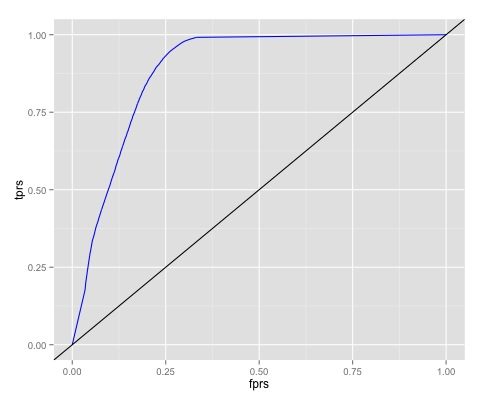
\includegraphics[scale=0.35]{plot/bestQDAfold1.jpeg} & 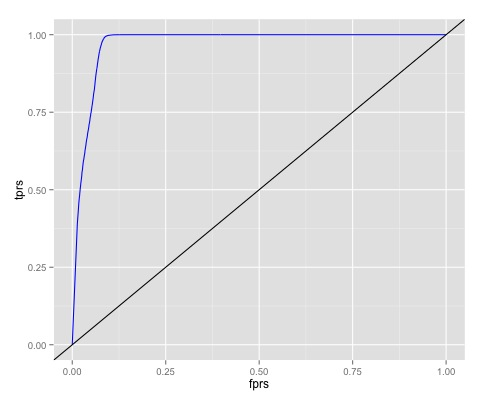
\includegraphics[scale=0.35]{plot/bestQDAfold2.jpeg}\tabularnewline
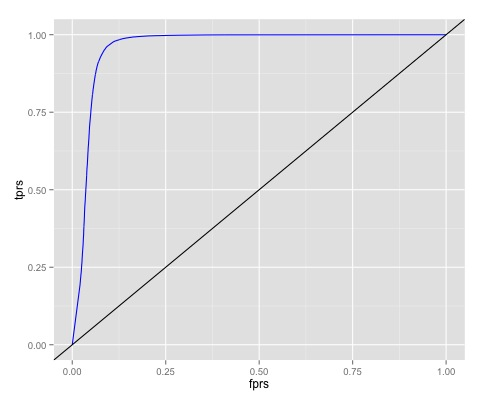
\includegraphics[scale=0.35]{plot/bestQDAfold3.jpeg} & 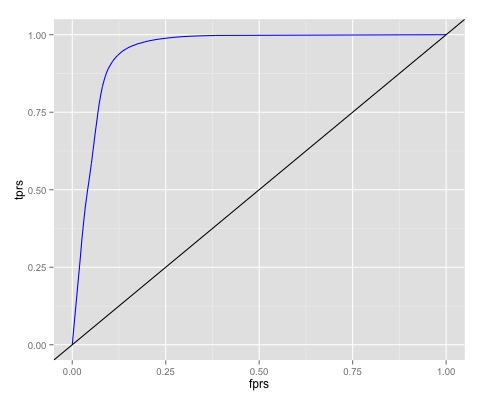
\includegraphics[scale=0.35]{plot/bestQDApooled.jpeg}\tabularnewline
\end{tabular}
\par\end{centering}

\protect\caption{ROC curves for QDA with NDAI, SD and CORR}


\end{figure}



\subsection{Model Assessment for SVM classifier}

The measures to validate the classification for different training
sizes are plotted in the figure below. It can be seen that across
different measures such as accuracy ((TP+TN)/(TP + TN + FP + FN)),
TPR (TP/(TP + FN)), FPR (FP/(FP + TN)) and FDR (FP/(FP + TP)), SVM
performs poorly as a classifier for the cloud data.\\
\begin{figure}[H]
\centering{}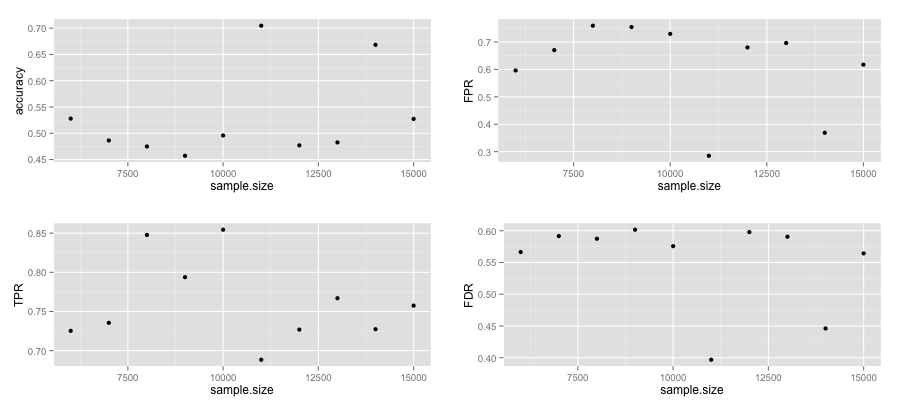
\includegraphics[scale=0.5]{plot/SVM_plots}\protect\caption{Model assessment for SVM}
\end{figure}

\noindent
It is surprising that these measures do not show a consistent trend
as the sample size increases, which may be accounted to the fact that
the strength of this classifier is largely dependent on how representative
the training set is. Since the sampling of the training set is random,
we can never be sure that the training data has a representative sample
of for both cloud and non-cloud. Since increasing the sample size
doesn\textquoteright t directly address this problem, we do not see
consistent trends of improvement in performance due to increase in
training sample size. Thus we do not consider the SVM classifier in
its current formulation as an appropriate model for classifying cloud
and non-cloud.


\section{Best Classification Model}

A closer look at the AUC from the logistic model, LDA and QDA makes
us think that there might be a better model that combines these two
models and gives us more stable prediction. Notice that QDA seems
to have the best performance by having the greatest average AUC as
well as joint AUC. However, QDA gives the worst AUC when predicting
for image3. In addition, logistic regression provides the best AUC
when predicting for image 3 but does not perform well for image 3.
Thus we propose that a more stable model can be achieved by giving
weights to the probability vectors predicted from the logistic model
and QDA. We do not include LDA because the performance of LDA is not
as good when predicting all three images.\\
\\
A naive model to consider is to weigh the probability vectors the
same, i.e. 0.5 on the logistic model prediction probability and 0.5
on the QDA logistic model prediction. We used this model and assess
the fit for the three folds. The AUC for the three folds are 0.8949305,
0.9639261and 0.9573461 respectively. The average AUC is slightly smaller
than the average AUC of the best QDA model but the variance of AUC
is smaller in this model, which demonstrate an improvement in stability.
Changing the weights on the two models does not change the result
too much since the AUC for both methods are similar to begin with.
Hence we will just work with the ensemble model with equal weights
on the probability vectors from the logistic model and QDA.\\
\\
We would use this model as our best model for predictions on new images
by training on all three images we have now.


\section{Misclassification Error Analysis}

In this section, we explore the misclassification error from the best
classification model. The following plots show the misclassification
locations, expert labels and the original image of image1. Note that
the same pattern is observed in the misclassification of the other
two images as well, so we show the plots for image3 as an example
since image3 has the biggest misclassification error. 

\begin{figure}[H]
\begin{centering}
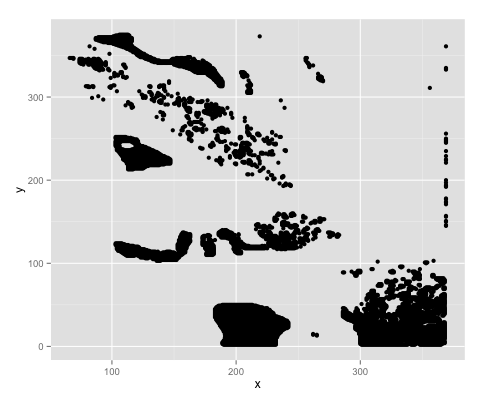
\includegraphics[scale=0.35]{plot/misclass11}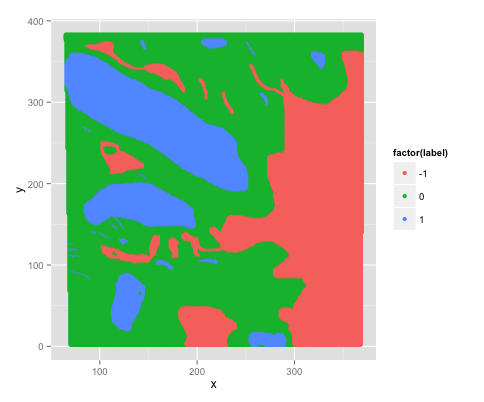
\includegraphics[scale=0.35]{plot/misclass12}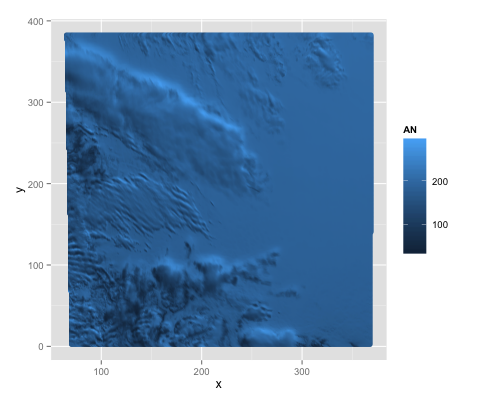
\includegraphics[scale=0.35]{plot/misclass13}
\par\end{centering}

\protect\caption{The left plot shows the pixels that are misclassified. The middle
plot shows the original expert labels. The right plot shows the actual
image from AN radiance.}
\end{figure}

\noindent
As we can see, the misclassification locations tend to cluster in
particular regions of the image. Misclassification happens when the
region is small and distant from the other regions with the same label.
Furthermore, misclassification locations are scattered at the pixels
with bigger variations in the region. Those variations may be the
landscape of the location.

\begin{figure}[H]
\begin{centering}
\begin{tabular}{ccc}
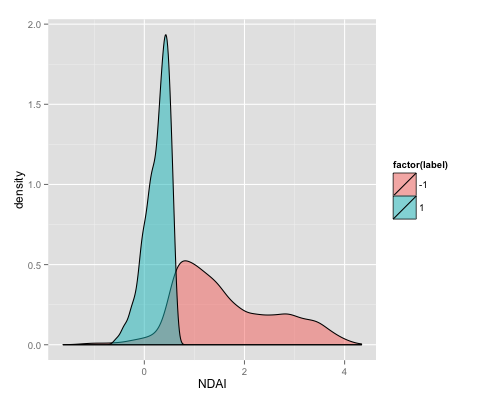
\includegraphics[scale=0.31]{plot/misclass14} & 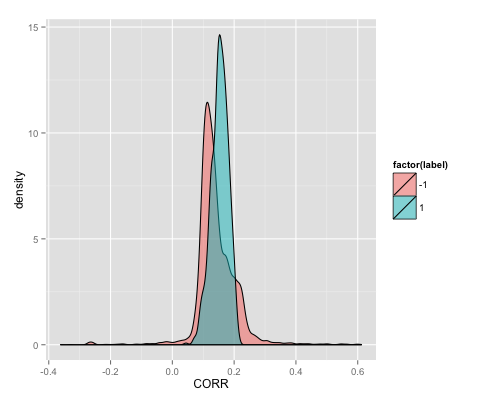
\includegraphics[scale=0.31]{plot/misclass16} & 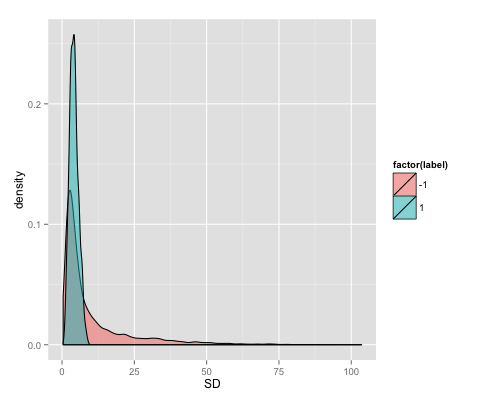
\includegraphics[scale=0.31]{plot/misclass18}\tabularnewline
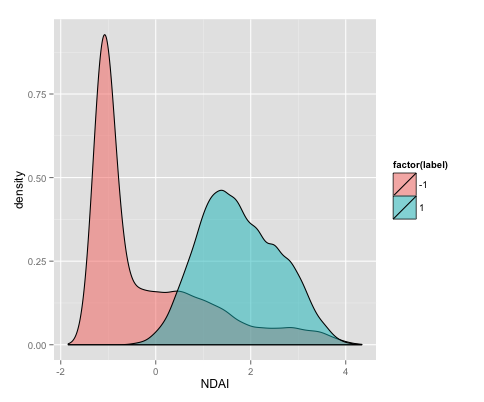
\includegraphics[scale=0.31]{plot/misclass15} & 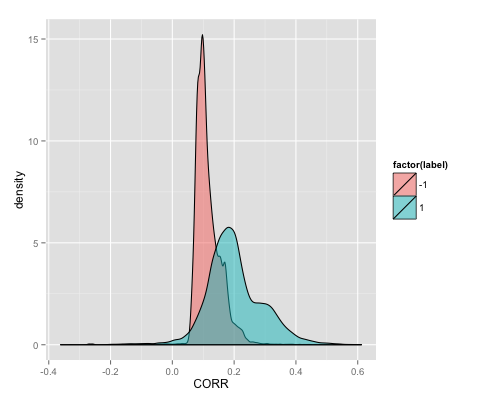
\includegraphics[scale=0.31]{plot/misclass17} & 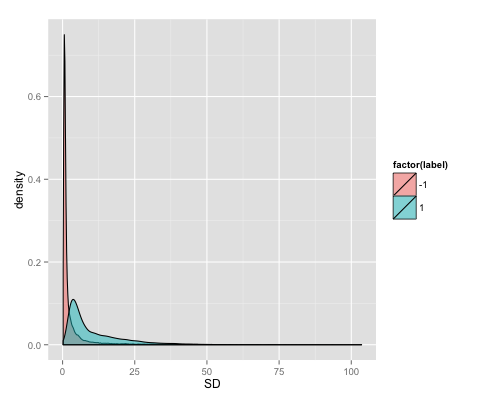
\includegraphics[scale=0.31]{plot/misclass19}\tabularnewline
\end{tabular}\protect\caption{The first row is the density plots of NDAI, CORR and SD of the misclassification
errors. The second row is the original density plots of NDAI, CORR
and SD of the same image.}

\par\end{centering}

\end{figure}

\noindent
By the density plots of the misclassification errors, we can see that
misclassification mainly happens in the intersection of cloud/no cloud
in the three featured values. This is reasonable because when our
model tries to find the probability of classification, the intersection
of values in the features are the hardest to separate. Hence misclassification
mainly occurs in those regions where the featured values are similar
but the labels are different.


\section{Future Prediction}

Future prediction is a very important aspect for choosing the best
classfiier model and is often ignored. The best models are chosen
based on the available data (cross-validating on training and test)
using measures such AUC, AIC and BIC. However, it is important to
remember that these measures indicate the accuracy of the model in
predicting for the type of data that is available before-hand. Future
prediction may be bad, if the image is very different from the data
that the classification was trained on.\\
\\
To account for such situations, we focused on the stability of AUC
across the different folds during our model selection. The average
AUC of our best classification model was slightly less than the average
AUC of its component QDA model. The better stability of the AUC over
different folds in the best classification model shows that the ensemble
model works better on new or different images than the QDA model.Since
future prediction is important for our classifier, we choose the ensemble
as our best model. Thus, our classification model is poised to work
well on future data without expert labels.\\
\\
In addition, our approach of choosing the cross-validation folds ensures
good future prediction. Since we trained our classification model
on two images and tested on the third, we have ensured that our model
is being tested on 'unseen' image and data points. Our best model
has been chosen from the performance of the models on the unseen images
in 3 folds and simulates the future prediction situations in which
we are given completely new images unseen by the classifier.
\begin{thebibliography}{1}
\bibitem{key-2}https://github.com/mozhou/cloud-data-lab\end{thebibliography}

\end{document}
